\section{Implementing Linux Personality}
\label{sec:graphene:background}

%Recent library OSes~\citep{porter11drawbridge,unikernels,baumann13bascule,osv}
%are designed for security and efficiency, but are limited to single-process applications.
%The security isolation of \liboses{} derives from 
%limited, explicit data sharing and 
%a narrow host interface.  
A \libos{} typically executes in either a paravirtual VM~\citep{unikernels,osv}
% \daniela{I would have the use of a VM as a discussion topic in the end of the paper.}, 
or an OS process, called a \term{\picoproc{}}~\citep{porter11drawbridge,baumann13bascule},
with an interface restricted to a narrowed set of host kernel ABIs.
These host ABIs heavily restrict effects outside of the application's address space;
as a result, applications in a \picoproc{} have very little opportunity to interfere with each other,
yielding security isolation comparable to a VM.
Library OS efficiency comes from deduplicating features, such as hardware management;
in a VM these features typically appear in both the guest and host kernels.


\sysname{} executes within a \picoproc{} (Figure~\ref{fig:graphene:arch}),
which includes an \term{unmodified} application binary and supporting libraries, 
running on a \libos{} instance.
The \libos{} is implemented over a host kernel ABI
designed to expose very generic abstractions that can be easily 
implemented on any host OS, including virtual memory, threads, synchronization, byte streams (similar to pipes),
a file system, and networking.
Although the \sysname{} prototype  host kernel is Linux, 
we adapt a host ABI from Drawbridge/Bascule,
which has been previously implemented on Windows, Hyper-V, and Barrelfish~\citep{porter11drawbridge,baumann13bascule,baumann09barrelfish}.
%The \sysname{} host ABI is
% summarized in Table~\ref{tab:abi} and discussed in more detail in \S\ref{sec:linux:pal}\fixmedp{if not cut...}.  
%which exposes only tens of simple host calls. \daniela{briefly define \picoproc{}: A \picoproc{} is unmodified application code running with a \libos{}.}


\begin{figure}[t]
\centering
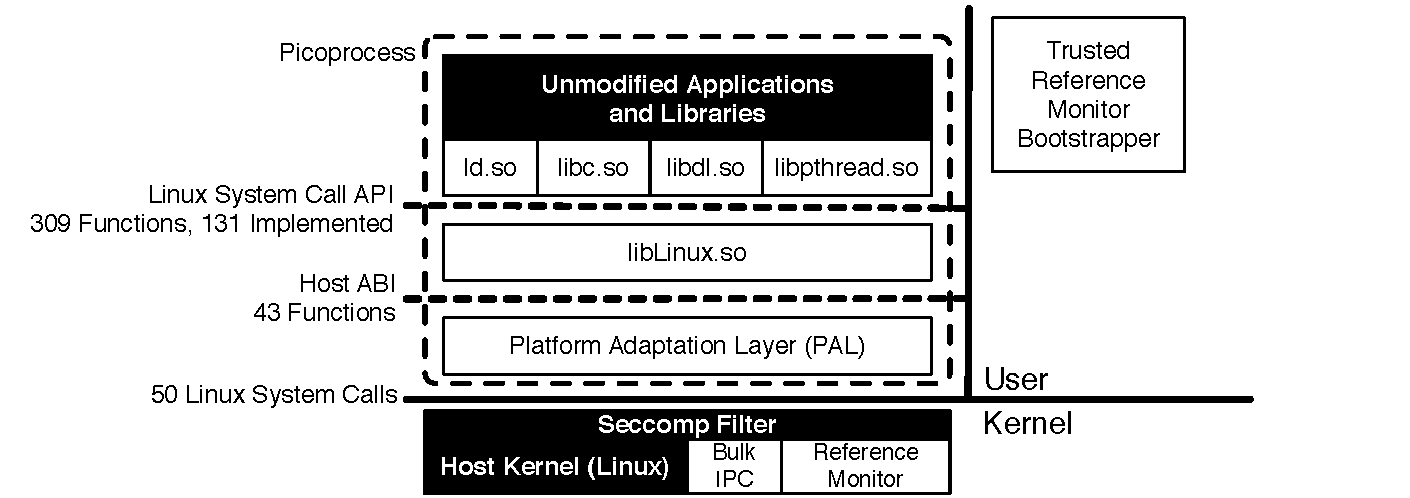
\includegraphics[width=6.5in]{graphene/figures/arch.pdf}
\caption[The \sysname{} building blocks]
{Building blocks of \sysname{}.  Black components are unmodified.
We modify the four lowest application libraries on Linux:
{\tt ld.so} (the ELF linker and loader),
{\tt libdl.so} (the dynamic library linker),
{\tt libc.so} (standard library C),
and {\tt libpthread.so} (standard threading library),
that issue Linux system calls as function calls directly to {\tt libLinux.so}.
Graphene implements the Linux system calls
using a variant of the Drawbridge ABI,
which is provided by the Platform Adaptation Layer (\pal{}),
implemented using calls to the kernel.
A trusted reference monitor that ensures \libos{} isolation
is implemented as a kernel module.
Another small module is added for fast bulk IPC.}
\label{fig:graphene:arch}
\end{figure}


\sysname{} exports \palcalls{} host ABIs through a 
Platform Adaptation Layer (\pal{}) (Table~\ref{tab:graphene:abi}).
The \pal{} is a binary injected into the \picoproc{} by the host, 
and translates the generic \picoproc{} ABI into host system APIs.
Most of these calls only affect the application-internal state;
any calls with external effects are mediated by a trusted \term{reference monitor} on the host.
%The reference monitor is a trusted non-\sysname{} process running on the system.
All \sysname{} applications are launched by the reference monitor,
which installs a system call filter and interposes on permitted kernel calls to ensure isolation
(\S\ref{sec:graphene:security}).


These \pal{} ABIs should be a sufficient substrate upon which to
implement guest-specific semantics, or guest \term{OS personality}.
As an example of this layering, consider the heap memory management abstraction.
Linux provides applications with a data segment---a 
legacy abstraction dating back to original Unix and the era 
of segmented memory management hardware.
The primary thread's stack is at one end of the data segment, and the heap is at another.  
The heap grows up (extended by {\tt sys\_brk}) 
and the stack grows down until they meet in the middle.
In contrast, the \pal{} ABI provides only three simple functions 
that allocate, protect, or unmap regions of virtual memory
with basic access permissions (read, write, and execute).
This clean division of labor encapsulates 
idiosyncratic abstractions in the library OS,
and eliminates the need for
redundant hardware management code, 
such as duplicate low-level page management and swapping heuristics.


%These interfaces are host-independent \daniela{OS or kernel-independent}, as they tend to be very generic and easily
%implemented on any host OS kernel or VMM \daniela{postpone VMM for later}.

At a high level, these library OS designs
scoop the layer just below the system call table out of the OS kernel
and refactor this code as an application library.  
The driving insight is that there is a natural, functionally-narrow division point 
one layer below the system call table
in most OS kernels.
Unlike many OS interfaces, these \pal{} ABIs generally minimize the amount of application state in the kernel, facilitating
migration: a \picoproc{} can programmatically read and modify its own OS state,
copy the state to another \picoproc{}, and the remote \picoproc{} can 
load a copy of this state into the OS---analogous to hardware registers.
A \picoproc{} may not modify another \picoproc{}'s OS state.



%% To implement the Linux OS
%% personality, we introduce 1 ABI for managing x86 segment registers and
%% 2 for handling runtime hardware exceptions.  The extensions are
%% expected to uphold host compatibility since they are also identified
%% and introduced in Bascule. In addition, 6 new ABIs, including
%% copy-on-write page exchanges, stream handle sharing, and sandbox
%% creation, are introduced to improve either efficiency or security
%% isolation of library OSes. These ABIs can always fall back to the
%% Drawbridge/Bascule ABIs if users decide to prioritize compatibility.

\begin{table}[t]
\footnotesize
\centering
\begin{tabular}{|l|c|>{\palign{l}}p{4.8in}|}
\hline
\multicolumn{3}{|c|}{\bf Adopted from Drawbridge} \\
\hline
{\bf Class} & {\bf ABIs} & {\bf Description} \\
\hline
Memory & 3 & Allocate and protect virtual memory. \\
\hline
Scheduling & 12 & Threads and synchronization. \\
\hline
Files \&  Streams & 12 & Files inside a {\tt chroot}-style; jails and byte streams among \picoprocs{}. \\
\hline
Process & 2 & Create a child \picoproc{}, and exit self. \\
\hline
Misc & 4 & Get random bits, time of day, etc. \\ % flush instruction cache, etc.\\
\hline
\multicolumn{3}{|c|}{\bf Added by \sysname{}} \\
\hline
{\bf Class} & {\bf ABIs} & {\bf Description} \\
\hline
Segments & 1 & Manage x86 segment registers (FS and GS) for TLS. \\
\hline
Exceptions & 2 & Handle hardware exceptions. \\
\hline
Streams & 4 & Share stream handles across \picoprocs{}, rename files, and set stream attributes (file permissions, socket options, etc.) \\
\hline
Bulk IPC & 3 & Exchange copy-on-write pages.\\
\hline
Sandboxes & 1 & Move into a new sandbox, with a new manifest applied. Pipes and streams that violates the new policy are closed.\\
\hline
\end{tabular}
\caption[List of host ABI functions defined in \sysname{}]
{Classes of  host ABI functions adopted from \drawbridge{}~\citep{porter11drawbridge}, 
followed by ABIs added by \sysname{}. \fixme{highlight difference with Bascule ABI}}
\label{tab:graphene:abi}
\end{table}


\fixme{Need transition to next section.}

\subsection{Multi-Process Support in Library OSes}

A key design feature of Unix is that users compose simple utilities to create
larger applications.  Thus, it is unsurprising that many popular applications for Unix or Linux
require multiple processes
--- an essential feature missing from current \libos{} designs.
%This gap is filled by the \sysname{} \libos{}, which
%extends recent \liboses{} to support multi-process applications.
The underlying design challenge is minimally expanding 
a tightly-drawn isolation boundary
without also exposing idiosyncratic kernel abstractions or
re-duplicating mechanisms \fixme{Discuss deduplicating features upfront} in both the kernel and the \libos{}.

%requires a careful balance among the competing goals of 
%efficiency, host independence, and security isolation.
%The challenge, then, is minimal expansion of

%\vspace{5pt}
%\noindent {\bf Motivating Example.~}
For example,
consider the process identifier (PID) namespace.
In current, single-process lib\-OSes, 
the {\tt getpid()} system call could simply return a fixed value to each application.
This  single-process design is isolated,
but the library OS cannot run a shell script, which requires {\tt fork}-ing and {\tt exec}-ing multiple binaries, signaling, waiting, and other
PID-based APIs.

\vspace{5pt}
\noindent{\bf Design Options.~}
Multi-process  support requires extensions to the \pal{} ABI of recent, single-process \libos{} designs.
Because multi-process abstractions, 
such as signals or System V IPC, 
tend to be idiosyncratic,
an essential problem is identifying a minimal, host-independent
substrate upon which 
to implement OS-specific abstractions.

We see two primary design options:
(1) implement processes and scheduling in 
the library OS, and (2) treat each \libos{} instance as a process, and distribute the 
shared POSIX implementation across a collection of \liboses{}.
We selected the second option, primarily because we expected this would impose fewer
requirements on the host, maximize flexibility in mapping processes 
to physical resources, and facilitate inter-process security policy enforcement. % as enforcing security policies on related processes.

Implementing processes
inside the library OS is also feasible using 
hardware MMU virtualization, similar to Dune~\citep{belay12dune},
but this reintroduces a duplicate scheduler and memory management.
Moreover, Intel and AMD have similar, but mutually incompatible MMU virtualization support,
which would complicate live migration across platforms.
None of these problems are insurmountable, and it would be interesting in future
work to compare both options.

\paragraph{Multi-Process Support in \sysname{}.}
%\daniela{Because Approach and Motivating Example are on the same level, its seems that
%you are starting a new topic under Approach, when the discussion is actually a continuation of
%Motivating Example}
In \sysname{}, multiple \libos{} instances in multiple \picoprocs{} collaborate to 
implement shared abstractions, such as 
 copy-on-write fork, signals, exit notification,
and System V IPC.
For instance, when process A signals process B on \sysname{}, A's \libos{} issues
a remote procedure call (RPC) to B's \libos{} over a host-provided byte stream (similar to a Unix pipe),
and B's \libos{} then calls the appropriate signal handler.

%%% All collaborating \libos{} instances exchange messages as needed 
%%% to provide the application with a consistent view of 
%%% shared abstractions,
%%% such as


%\sysname{} approaches multi-processing by selectively replicating state and issuing remote procedure calls (RPCs) 
%%across multiple, collaborating
%library OS instances.
%Guests may work together to provide the unmodified multi-process application with
%coordination abstractions 

%Shared abstractions on \sysname{}'s are implemented outside of the host, ensuring  host OS independence.
% by implementing these
%shared abstractions entirely
%outside of the host kernel.
%Shared abstractions are implemented outside of the host.
%From the host kernel's perspective, 
\sysname{} implements all shared abstractions in the \libos{}, and \liboses{} cooperatively manage these abstractions
over RPC streams.
Single-process applications still service system calls from local state, and \sysname{} 
includes optimizations to place state where it is most likely to be used,
minimizing RPC overheads.
The host reference monitor can easily isolate \liboses{}
by 
% \sysname{} design isolates \liboses{} by 
%requiring all coordination to use 
%explicit bytes streams \daniela{, pipe-like abstractions provided by the kernel. (suggestion: Reviewer  3)}.
%Security isolation is enforced
%by a kernel-level {\em reference monitor}, which can 
%disconnect or prevent creation of a
blocking all
RPC messages, % between \liboses{} that should be isolated,
without the need to understand the \libos{} details or semantics of these abstractions.
In our PID example, only mutually-trusting \liboses{} can signal each other.
%if the reference monitor prevents creation of RPC streams
%across mutually untrusting \picoprocs{},
%the \liboses{} cannot exchange signals.

%%% \sysname{} is designed to 
%%% The \sysname{} design leverages a number of optimizations to service application system calls 
%%% from local state whenever possible, and to minimize message passing overheads otherwise
%%%  (\S\ref{sec:namespaces:insights}).
%%% Our experience is that starting with a local system call design and then extending it to share state is relatively straightforward,
%%% and introduces little-to-no overhead when the request can be serviced locally.


The \sysname{} library OS is designed
to gracefully handle disconnection from other \liboses{}, 
facilitating dynamic application sandboxing.
RPC streams may be disconnected at any time by 
either the reference monitor or at the request of a \libos{}.
%Message streams may be severed externally, by the reference monitor, or 
%one guest may simply disconnect from others to isolate itself.
%An application may disconnect itself from the 
%Any \sysname{} application may dynamically detach from the confederation, 
%or a host-level sandbox may dynamically separate two guests by severing their communication channels.
When \sysname{} \liboses{} are disconnected, each instance will handle the subsequent
divergence 
%and the library OS will will fork these abstractions
{\em transparently} to the application.
For instance, if a child process is disconnected from the parent by the reference monitor,
each \libos{} will interpret the event as if the other process terminated---closing any open pipes,
delivering exit notifications, etc.
% \daniela{(applications run unmodified) - Reviewer 1 asked clarification on transparently}.

%% A key insight behind our design is that the common use case for these \daniela{cooperating} abstractions
%% is between a pair of processes.  Thus \sysname{} leverages a number of optimizations 
%% to reduce broadcast messages, avoid replication of needless state,
%% and service requests locally


\paragraph{Changes to \pal{} ABI.}
When implementing \sysname{},
we found that the Drawbridge ABI lacked 12 \pal{} calls
essential to running a Linux \libos{} with multi-process support, and 
\sysname{} did not require 3 \pal{} calls to support checkpoint and resume.
Of the 12 new calls, 4 are required for single-process Linux and similar ABI have also been added by \term{Bascule}~\citep{baumann13bascule}:
rename a file, manage segmentation hardware, and 2 for exception upcalls;
5 are required for stream inheritance, attribute configuration, and sandboxing;
and 3 new calls are used to utilize Bulk IPC channel, for optimizing copy-on-write fork (\S\ref{sec:graphene:impl}).
%Our design requires only 11 additional \pal{} calls, which we believe are fundamental to executing 
%Unix-style multi-process applications.
We design these new \pal{} calls in consideration of the platform independence
among different hosts;
If a \pal{} call is added for optimizations (e.g., Bulk IPC),
it is optional if the implementation is difficult or infeasible on a host.
%in case that the new \pal{} calls are not possible to implement on a host,
%the 
%Our design deliberately provides options where these new \pal{} calls are missing, to preserve the platform importance proven by \term{Drawbridge}~\citep{porter11drawbridge}.
For example, copy-on-write forking can still be supported
without Bulk IPC supported on the host.
Instead, the inheritance of process state for
copy-on-write forking will be completely over regular pipes.

\paragraph{Comparison with \microkernel{}s.}
The building blocks of \sysname{} are very similar to the system abstractions of a 
\microkernel{}~\citep{liedtke95sosp,klein09sel4,elphinstone13microkernels,liedtke93sosp,chen93memory,Baron:1985:MOE,Accetta:1986:MNK},
except a \microkernel{} often has a even narrower, more restricted interface
than the \pal{} ABI.
%such as the port and
%message abstractions of Mach~\citep{
Unlike a multi-server \microkernel{} system, such as GNU Hurd~\citep{hurd} or Mach-US~\citep{stevenson95mach-us},
which implements Unix abstractions across a set of daemons that are shared by all processes in the system,
\sysname{} implements system abstractions as a library in the application's address space,
and can coordinate library state among \picoprocs{} to implement shared abstractions.
\sysname{} guarantees isolation equivalent to running 
an application on a dedicated VM; this isolation could be implemented on a multi-server \microkernel{}
by running a dedicated set of service daemons for each application.

%%% \sysname{}'s differences are motivated by two considerations: efficient support of both stand-alone, 
%%% single-process applications and multi-process applications; as well as flexible security isolation. 
%%% \sysname{} contributes techniques to seamlessly and efficiently transition 
%%% between single-process and multi-process support, as well as adapting 
%%% some known techniques to a new environment.

The \sysname{} host ABI could be described as a hybrid \microkernel{},
which also exposes the file system and network of the host kernel.
Similarly, we assume that \picoprocs{} are provided by a legacy OS kernel, like Linux or Windows,
or by a Type 2 hypervisor.  We expect that a bare metal hypervisor could export a \pal{},
but would probably require services from a trusted VM, such as Xen's dom0~\citep{barham03xen}.
%or the \pal{} would implement more thread scheduling, networking, and file system code;
%or the \pal{} ABI would change to push this code into the \libos{}.
Arguably, recent \libos{} designs might be improved by rethinking the division of labor in
the network and file system stacks, but this is beyond the scope of this thesis.

\paragraph{Alternatives.}
Another approach to support multi-process applications in a \libos{} 
would be to use hardware MMU virtualization such as nested paging
used by a system like Dune~\citep{belay12dune}
in order to implement a second process abstraction, memory manager, and scheduler in the \libos{}.
This approach threatens the efficiency benefits of deduplicating these features.
A final option is exposing additional kernel interfaces, such as signals, 
by adding more system calls to a \picoproc{}.
This approach undermines host independence, as many of these coordination abstractions 
tend to be very OS-specific.
%Unix signals vs.\ Windows events, {\tt waitpid()} vs.\ blocking on a process handle, etc.
This approach also harms security isolation, as the \libos{} now has access to generally 
porous host kernel interfaces.  
%Although legacy OSes do enforce some access control rules on coordination abstractions,
%kernel developers must audit and add hooks to millions of lines of code.
%As a result,
%users have lost confidence that a traditional OS can comprehensively enforce 
%security isolation on these abstractions---a key motivation for using VMs
%for security isolation.


Systems must strike a careful balance between the competing goals of
security isolation and
multi-process coordination.
Multi-process applications require OS-managed coordination abstractions
such as signals, process exit notification, and System V IPC.
These coordination abstractions operate within shared namespaces, such as the 
process ID namespace
and the System V key space.
These coordination APIs and namespaces must be consistent among coordinating processes,
but can %introduce information leaks and 
undermine security isolation among unrelated processes on the same host.
System designs generally only meet one goal: 
traditional OSes have a rich but porous coordination interface, 
while sandboxing systems and virtual machines (VMs) 
are strictly isolated.
This thesis demonstrates that this unfortunate trade-off is not
fundamental.
%coordination or isolation.  


Traditional OS kernels typically provide  rich multi-process coordination 
APIs, but this richness also makes for a very porous attack surface
area.  For instance, on Windows, a program may inject libraries and
create threads in another program~\citep{windows-dll-inject}; 
similarly, unchecked file descriptor inheritance in Linux can lead to
security problems~\citep{close-on-exec}.  
Although legacy OSes do enforce some access control rules on these abstractions,
kernel developers must audit and add hooks to so much code
that
users have lost confidence that an OS can comprehensively enforce 
security isolation on these abstractions.

For achieving strong security isolation on applications,
%generally lost confidence that legacy OSes can robustly enforce security isolation, and 
users have turned to virtual machines (VMs).
For instance, if two customers host their websites in the same cloud service,
the customers will insist on running their web servers in separate VMs for security.
VMs take a heavy-handed approach to security isolation --- ensuring 
that every application has a dedicated OS kernel in a hardware-isolated address space.
Although virtual machines isolate
applications and provide legacy OS abstractions within a VM, 
coordinating applications must be statically placed in the same VM,
and cannot dynamically move to a separate VM.
For instance, consider a web service running
inside of a VM that wishes to isolate requests for different users in
different VMs after authentication.  The web server administrator must
statically create a VM for each user, introducing substantial
overhead; and the developer loses convenient IPC abstractions and
must rewrite large swaths of code.
